\section{Introduction}


Aligning Large Language Models (LLMs, ~\citealt{brown2020language,chowdhery2023palm, touvron2023llama,achiam2023gpt}) with human ethical standards and practical expectations is extremely crucial to prevent unintended consequences and ensure AI's positive contribution to society. Traditional alignment methods, such as supervised fine-tuning (SFT) and reinforcement learning from human feedback (RLHF)~\cite{bai2022constitutional, ouyang2022training}, are resource-intensive and require extensive human oversight, limiting their scalability and practicality. As LLMs grow more complex and widely adopted, the demand for cost-effective, annotation-efficient, and rapidly adaptable alignment strategies becomes increasingly urgent.



% \vspace{-5pt}
\begin{figure}
    \centering
    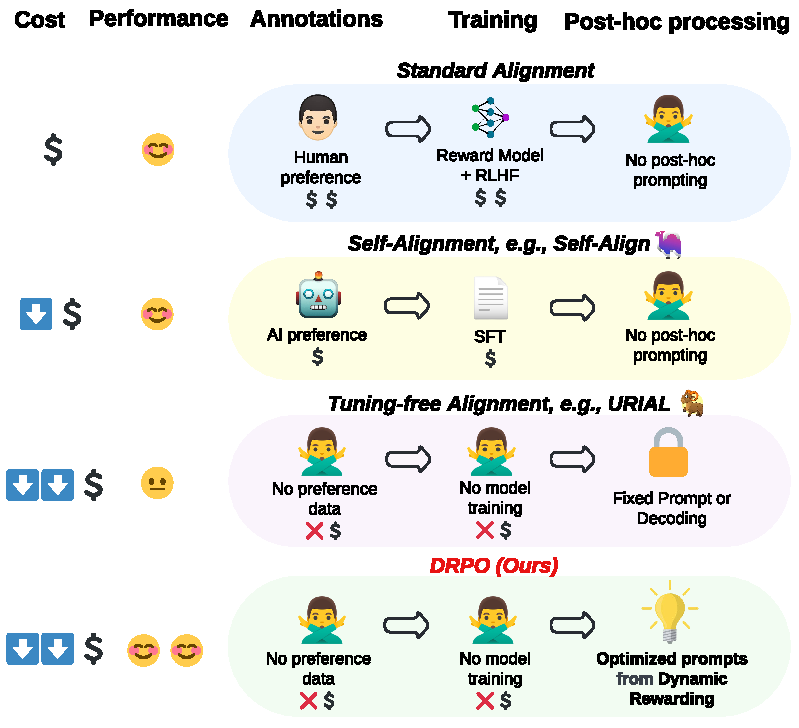
\includegraphics[width=1\linewidth]{images/DRPO_comparison.pdf}
    \vspace{-18pt}
    \caption{Comparison of \ours with other LLM alignment paradigms. \ours combines the benefits of self-alignment and tuning-free alignment, enabling self-improvement and high cost-efficiency without requiring human supervision or additional model training.
    }
    \vspace{-22pt}
    \label{fig:paradigm_comparison}
\end{figure}



Self-alignment aims to improve LLM alignment by leveraging the models themselves; for example, by replacing human feedback with model-generated feedback~\cite{lee2023rlaif}, synthesizing preference data~\cite{kim2023aligning, sun2024principle}, or self-critique~\cite{bai2022constitutional}. Despite these advancements, such methods still demand significant resources, including the costly and unstable RLHF tuning, as well as some level of human supervision, such as carefully curated alignment rules or in-context learning (ICL) prompts~\cite{sun2024principle}. On the other hand, as shown in Figure~\ref{fig:paradigm_comparison}, a recent line of research focuses on tuning-free alignment, which prioritizes extreme efficiency without incurring any tuning cost. These approaches include techniques like decoding-based alignment~\cite{li2023rain, wang2024inferaligner} or ICL alignment~\cite{han2023context, Lin2024ReAlign, zhao2024context}. However, these tuning-free methods are often static (e.g., relying on fixed prompts or reward functions) and thus lack the flexibility to adapt and self-improve for better alignment. 




To marry the strengths of both paradigms, in this paper, we propose \ours, Dynamic Rewarding with Prompt Optimization, a novel tuning-free approach for LLM self-alignment. \ours draws inspiration from two key insights from recent alignment research. First, the superficial alignment hypothesis~\cite{zhou2024lima} suggests that LLMs can be effectively aligned through lightweight tuning or even simple prompting~\cite{Lin2024ReAlign, zhao2024context}. Second, reward models in RLHF often generalize poorly to out-of-distribution samples~\cite{burns2023weak}, whereas LLMs, known for their superior generalization capabilities, can provide more effective rewards and feedback for alignment purposes. Building on these insights, \ours is constructed atop a search-based prompt optimization (PO) framework~\cite{pryzant2023automatic, hao2023reasoning, wang2023promptagent}, which enables LLMs to self-correct and automatically craft detailed alignment instructions. This steers model behavior more effectively, without relying on any use of human preferences or model training. 




The core novelty of \ours lies in its \textit{dynamic rewarding} mechanism, integrated with the optimization framework. This mechanism allows LLM-based rewards to be dynamically adjusted based on specific queries, helping to identify and address the model's alignment blind spots. For example, if an LLM with outdated knowledge pretends to answer a question requiring the latest news, its ``knowledge limitation'' reward will be low, and the alignment prompt will be updated accordingly. We apply this novel method to automatically craft both the system prompt and responses in ICL examples, which have proven highly effective in improving alignment.




We conducted comprehensive experiments on 8 recent LLMs using the standard alignment benchmark, \texttt{just-eval-instruct}, composed of questions from multiple alignment datasets. Our results show that \ours can effectively align both base and SFT/RLHF tuned models. Notably, \ours significantly enhances base models, enabling them to outperform their SFT/RLHF-tuned counterparts. \ours can further improve SFT/RLHF-tuned models, highlighting its compatibility with other tuning-based alignment techniques. Additionally, our automatically optimized prompts substantially outperform those curated by human experts. 





\begin{figure}
    \centering
    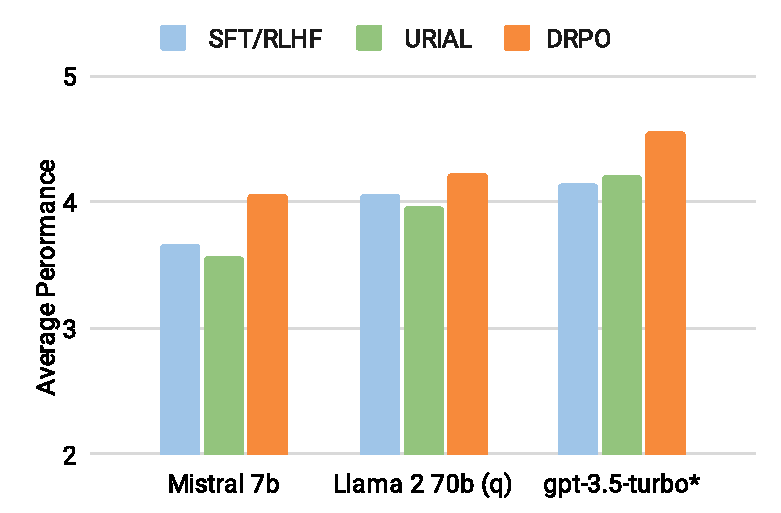
\includegraphics[width=1.0\linewidth]{images/method_comparison_column_chart_white_bg.pdf}
    \vspace{-15pt}
    \caption{Comparison of \ours with other alignment methods, including RLHF and URIAL~\cite{Lin2024ReAlign}. \ours consistently outperforms both baselines across multiple LLMs.
    Note that we do not have access to \texttt{gpt-3.5-turbo} base model; hence, both \ours and URIAL are directly applied to its RLHF-tuned version.}
    \label{fig:overall_comparison_chart}
    \vspace{-15pt}
\end{figure}












